	\documentclass[12pt,a4paper,italian]{article}


\usepackage[italian]{babel}
\usepackage[latin1]{inputenc}
\usepackage{amsmath}
\usepackage{amsfonts}
\usepackage{amssymb}
\usepackage{color}
\usepackage{xcolor}
\usepackage{hyperref}
\usepackage[all]{hypcap}
\usepackage{ifthen}
\usepackage{wrapfig}
%\author{Piero Bizzotto}
\usepackage[top=2cm,bottom=5cm,left=80pt,right=80pt]{geometry}
\usepackage{graphicx}
\DeclareGraphicsExtensions{.jpg,.png}

\newcommand{\ajax}{AJAXDRAW}
\newcommand{\sito}{\href{http://ajaxdraw.sourceforge.net}{http://ajaxdraw.sourceforge.net}}

\setlength{\parindent}{0pt} %settato indentazione di default 
\setlength{\headheight}{3cm} %settato grandezza header...in altre parole, quanto distanzio il doc dall'intestazione

\usepackage{fancyhdr} %pacchetto per le intestazioni
\pagestyle{fancy} %uso del pacchetto


\fancyhead{} %annulla head di default
\fancyfoot{} %annulla foot di default


\usepackage{lastpage} %setto pg di pgtot a rfoot
     \rfoot{pagina \thepage\ di \pageref{LastPage}}


\lfoot{Versione: \insertversion} %setto versione doc a lfoot
\renewcommand{\footrulewidth}{0.5pt} %ridefinisco il valore della riga di intestazione
\renewcommand{\headrulewidth}{0.5pt} %ridefinisco il valore della riga di pie' di pagina

\newcommand{\insertversion}{0.0} %definisco il nuovo comando per inserire la versione


\lhead{  \begin{Huge} \ajax \end{Huge} \\  %intestazione di sinistra
					%\begin{Large}	Software per il Disegno Grafico\\ in Tecnologie Web \end{Large}  
					\begin{normalsize}\sito \end{normalsize}
			%\\ versione documento: \insertversion\ del \today} %setto l'intestazione sx
		}
\rhead{ %includo logo nell'intestazione dx
	 	
\includegraphics[scale=0.5]{../logo/logo}  
}


%CREAZIONE ELENCHI NUMERATI PERSONALIZZATI
\newcounter{Lcount}
\newcounter{Rcount}
\setcounter{Lcount}{0}
\setcounter{Rcount}{0}

\newenvironment{elenconumerato}[2][ ]
{
  \begin{list}{#1\arabic{Lcount}.}
    {
	\setcounter{Rcount}{\value{Lcount}}
	\setcounter{Lcount}{0} 
	\usecounter{Lcount} 
\addtolength{\leftmargin}{#2pt}
	}
}
{
  \end{list}
 \setcounter{Lcount}{\value{Rcount}}
}

%CREAZIONE ELENCHI PUNTATI
\newenvironment{elencopuntato}[1][]
{
\begin{list}{\textbullet} %\itemindent=#1pt
	{
	\addtolength{\leftmargin}{#1pt}
	}
} 
{
\end{list}
}


\newenvironment{elencodescrittivo}[1][]{\begin{description} \setlength{\itemindent}{#1pt} \addtolength{\leftmargin}{#1pt}} {\end{description}}

\newcommand{\TITOLODOC}{Titolo}

%footer centrale
\cfoot{ \TITOLODOC \\  E-mail:    \href{ mailto:webshape.contact@gmail.com}{ webshape.contact@gmail.com}  }

%INSERIMENTO IMMAGINI
\newcommand{\imagerealsize}[1]{\vspace{20pt} \includegraphics{#1} }
\newcommand{\imageadapted}[1]{\vspace{20pt} \includegraphics[width=1\textwidth]{#1} }

\newcommand{\glosspath}{.\glossario}
\newcommand{\gloss}[1]{\hyperref{\glosspath~\glossario.pdf}{}{#1}{#1}}

\hypersetup{
    %bookmarks=true,         % show bookmarks bar?
    %unicode=false,          % non-Latin characters in Acrobat’s bookmarks
	%pdftoolbar=true,        % show Acrobat’s toolbar?
	%pdfmenubar=true,        % show Acrobat’s menu?
    %pdffitwindow=true,      % page fit to window when opened
    %pdftitle={My title},    % title
    %pdfauthor={Author},     % author
    %pdfsubject={Subject},   % subject of the document
    %pdfnewwindow=true,      % links in new window
    %pdfkeywords={keywords}, % list of keywords
    colorlinks=true,         % false: boxed links; true: colored links
    linkcolor=black,           % color of internal links
    %citecolor=green,        % color of links to bibliography
    %filecolor=magenta,      % color of file links
    urlcolor=teal    % color of external links
%	linktocpage=false;
}


%COLORAZIONE TESTO
\newcommand{\blue}[1]{{\color {blue} #1}} 
\newcommand{\red}[1]{{\color {red} #1}}
\newcommand{\green}[1]{{\color {green} #1}}
\newcommand{\sezione}[1]{\leftskip=0pt \section{#1} \leftskip=18pt}
\newcommand{\subsezione}[1]{\leftskip=18pt \subsection{#1} \leftskip=36pt}
\newcommand{\subsubsezione}[1]{\leftskip=36pt \subsubsection{#1} \leftskip=54pt}
\newcommand{\subsubsecindent}{54}
\newcommand{\subsecindent}{36}
\newcommand{\secindent}{18}
\newcommand{\normindent}{8}
\newcommand{\code}[1]{{\bfseries \texttt{#1}}}
\newcommand{\paragrafo}[1]{\leftskip=36pt \paragraph{#1} \leftskip=54pt}
\newcommand{\subparagrafo}[1]{\leftskip=54pt \subparagraph{#1} \leftskip=72pt} %BASE!!!

\title{\TITOLODOC}
\author{Cunico Marco}

\begin{document}

\renewcommand{\insertversion}{0.7} %INSERIRE LA VERSIONE QUI DENTRO STILE x.x.xx
\renewcommand{\TITOLODOC}{Piano di Progetto} %INSERIRE IL TITOLO DEL DOCUMENTO DA FAR COMPARIRE A PIE PAGINA
\renewcommand{\glosspath}{.\glossario} %INSERIRE PERCORSO RELATIVO

%%%%%%%%%%%%%%%%%%%%%%PARTE DA NON MODIFICARE%%%%%%%%%%%%%%%%%
\begin{titlepage}
\begin{center}
	\begin{Large}	\today \end{Large}
\end{center}

\vspace{20pt}

\begin{center}
	\begin{Huge}
				\textbf{\ajax}
	\end{Huge}
\end{center}			

\begin{center}
	\begin{large}
				\textbf{Software per il Disegno Grafico in Tecnologie Web}
	\end{large}
\end{center}			

\vspace{20pt}

\begin{center}

\includegraphics[width=150pt]{../logo/logo}
\end{center}

\vspace{170pt}
\begin{center} %INSERIRE ALL'INTERNO IL TITOLO DOCUMENTO CHE COMPARIRA NELLA PAGINA INIZIALE				
	\begin{Huge}
				\textbf{\TITOLODOC}
	\end{Huge}
			\\
\end{center}
\vspace{210pt}
\begin{center}
Versione: \insertversion
\end{center}
\end{titlepage}

\newpage
%%%%%%%%%%%%%%%%%%%%%%FINE PARTE DA NON MODIFICARE%%%%%%%%%%%%%%%%%

\begin{center} %INSERIRE ALL'INTERNO IL TITOLO DOCUMENTO CHE COMPARIRA NELLA PAGINA INIZIALE
	\begin{Huge}	
				\textbf{\TITOLODOC}
			\\
	\end{Huge}
\end{center}

%\setlength{\parindent}{18pt} %settato indentazione di default 
\section*{\Large Sommario:}
Il presente documento descrive l'analisi dei costi e delle risorse effettuata dall'azienda WebShape per lo sviluppo del Capitolato C04.

 %SEZIONE SOMMARIO
\indent \indent

\section*{\Large Stato del documento:}
\indent \indent
	Formale Esterno

\section*{\Large Redazione:}
	\begin{elencopuntato}[\normindent]
		\item Cunico Marco
		\item Dal Bosco Davide
	\end{elencopuntato}

\section*{\Large Approvazione:}
	\begin{elencopuntato}[\normindent]
		\item Approvatore N. 1
		\item Approvatore N. 2
		\item Approvatore N. 3
	\end{elencopuntato}

\section*{\LARGE Lista di Distribuzione:}

	\begin{elenconumerato}{\normindent}
		\item WebShape 
		\item I committenti Vardanega Tullio e Conte Renato in rappresentanza \\  dell'azienda proponente Zucchetti SPA
	\end{elenconumerato}

\newpage



\section*{\Large Registro delle Modifiche:}


\begin{center}
	\begin{table}[h]
		  \begin{tabular*}
			{1\textwidth}%
				{@{\extracolsep{\fill}}|p{0.1\textwidth}|p{0.54\textwidth}|p{0.26\textwidth}|}
			 \hline
%%%%%%%%%%%%%%INTESTAZIONE COLONNE%%%%%%%%%%%%%%%%%%%%%%%%%%%%%%%%%%%%%%%%%%
			\textbf{Versione}  & \textbf{Descrizione} & \textbf{Autore} \\
%%%%%%%%%%%%%%FINE INTESTAZIONE COLONNE%%%%%%%%%%%%%%%%%%%%%%%%%%%%%%%%%%%%%%%
		 \hline
%%%%%%%%%%% PARTE DA MODIFICARE %%%%%%%%%%%%%%%%%%%%%%%%%%%%%%%%%%%%%%%%%%%
          0.7 & 05/12/2008 Inserimento Distribuzione Ruoli e Gestione del Piano di Progetto & Cunico Marco \\
          0.6 & 05/12/2008 Inserimento Preventivo Rotazione Ruoli per fase di progetto & Cunico Marco \\
          0.5 & 05/12/2008 Inserimento della sezione relativa all'Analisi e Gestione dei Rischi & Dal Bosco Davide \\         
          0.4 & 04/12/2008 Inserimento attribuzione ruoli & Cunico Marco \\	
%%%%%%%%%%% PARTE DA MODIFICARE %%%%%%%%%%%%%%%%%%%%%%%%%%%%%%%%%%%%%%%%%%%%%%%%%%		
          
          0.3 & 04/12/2008 Inserimento intero capitolo Pianificazione con relative sottosezioni,tabelle e grafici & Dal Bosco Davide \\
    	  0.2 & 01/12/2008 Inserimento capitoli Introduzione,Organigramma,Pianificazione(inizio) & Dal Bosco Davide \\
    	  0.1 & 25/11/2008 Adattamento al template scelto & Dal Bosco Davide \\
    	  0.0 & 22/11/2008 Bozza iniziale & Dal Bosco Davide \\

		\hline %%FINE RIGA
%%%%%%%%%%% FINE PARTE DA MODIFICARE %%%%%%%%%%%%%%%%%%%%%%%%%%%%%%%%%%%%%
		\end{tabular*}
	\caption{Registro delle modifiche} %INSERIRE DIDASCALIA - SE NECESSARIA - 
	\label{tab:modifiche}
	\end{table}
\end{center}


\newpage
\thispagestyle{fancy}
\tableofcontents
\thispagestyle{fancy}
\newpage

\sezione{Introduzione}

\subsezione{Scopo del documento}
Il documento si propone di presentare ai Committenti le scelte effettuate riguardanti la distribuzione dei ruoli e delle risorse, l'assegnazione delle attivit\`a dei componenti dell'azienda e lo studio dei costi necessari per la realizzazione del progetto inerente al capitolato d'appalto C04.\\

\sezione{Organigramma}
In data 15 ottobre 2008 \`e stato costituito il gruppo WebShape formato da sei membri, tutti in possesso delle idoneit\`a necessarie per partecipare al progetto di Ingegneria del Software.
I ruoli saranno assegnati a rotazione nell'arco dello sviluppo del progetto, in base alle capacit\`a e alle disponibilit\`a dei componenti del gruppo.\\

\subsezione{Accettazione}
\begin{table}[h]
	\begin{center}
		  \begin{tabular}{|p{0.3\textwidth}|l|p{0.3\textwidth}|}
		 \hline 
		 \textbf{Cognome e Nome} & \textbf{Data} & \textbf{Firma}\\
		 \hline
		Bizzotto Piero & 15-10-2008 & \\
		\hline
		Carollo Mirko & 15-10-2008 & \\
		\hline
		Cunico Marco & 15-10-2008 & \\
		\hline
		Dal Bosco Davide & 15-10-2008 & \\
		\hline
		Dissegna Stefano & 15-10-2008 & \\
		\hline
		Geremia Mirco & 15-10-2008 & \\
		\hline
		\end{tabular}
	\caption{Accettazione} 
	\label{tabella_accettazione}
	\end{center}	
\end{table}



\subsezione{Descrizione Componenti}
Vedere Tabella: (\ref{tab:tabella_componenti}) della pagina ~\pageref{tab:tabella_componenti}\\

\subsezione{Assunzioni Iniziali}
Regole da rispettare per la realizzazione del progetto didattico:
\begin{elenconumerato}{\normindent}
				\item L'importo totale stimato \`e di 13059 euro.\\
				\item Sono state previste 630 ore di lavoro.\\
				\item L'impegno individuale di ogni componente varia da un minimo di 85 ore ad un massimo di 105 ore.\\
			\end{elenconumerato}

\begin{table}[h]
	\begin{center}
		  \begin{tabular}{|p{0.3\textwidth}|l|l|}
		 \hline 
		 \textbf{Cognome e Nome} & \textbf{Matricola} & \textbf{E-mail}\\
		 \hline
		Bizzotto Piero & 540804 & piero.bizzotto@gmail.com \\
		Carollo Mirko & 542902 & mirko.carollo@gmail.com\\
		Cunico Marco & 540754 & marco.cunico@gmail.com\\
		Dal Bosco Davide & 539402 & mrdavi86@gmail.com\\
		Dissegna Stefano & 561011 & stefano.dissegna@gmail.com \\
		Geremia Mirco & 563665 & crittico@gmail.com\\
		\hline
		\end{tabular}
	\caption{Descrizione dei Componenti} 
	\label{tab:tabella_componenti}
	\end{center}	
\end{table}



\subsezione{Attribuzione dei Ruoli}
Date le Assunzioni Iniziali precedentemente descritte, ed essendo il gruppo WebShape costituito da sei membri, si avr\`a una media di circa 105 ore di lavoro per persona. La durata complessiva del progetto sar\`a di circa 630 ore, ogni componente lavorer\`a quindi una media di 3 ore giornaliere. Sono previste altre 3 revisioni:
\begin{elenconumerato}{\normindent}
				\item Revisione di Progetto Preliminare (RPP)
				\item Revisione di Qualifica (RQ)
				\item Revisione di Accettazione (RA)
			\end{elenconumerato}

La rotazione dei ruoli avviene come da tabella (\ref{tab:TabellaRotazRuoli}) della pagina ~\pageref{tab:TabellaRotazRuoli}.\\
Dato che ogni componente del gruppo dovr\`a assumere tutti i ruoli,\`e previsto che nelle varie fasi del progetto i membri della societ\`a si assumano piu' incarichi. Non \`e permesso che uno stesso membro ricopra ruoli in conflitto di interessi tra loro.\\
La rotazione dei ruoli avviene come da tabella (\ref{tab:tavprevrotazione}) della pagina ~\pageref{tab:tabprevrotazione}.\\
Dato che ogni componente del gruppo dovr\`a assumere tutti i ruoli, \`e previsto che nelle varie fasi del progetto i membri della societ\`a si assumano piu' incarichi. Non \`e permesso che uno stesso membro ricopra ruoli in conflitto di interessi tra loro.\\

\sezione{Pianificazione}
Per la realizzazione del progetto l'azienda WebShape ha valutato con attenzione i possibili modelli di cicli di vita da utilizzare, tenendo conto di eventuali pregi e difetti. 
La scelta \`e ricaduta sul modello incrementale, in quanto, vista la tipologia modulare del progetto, si adatta meglio alle esigenze dell'azienda stessa. Con il modello incrementale si ha la possibilit\`a di effettuare dei rilasci di versioni parziali in modo da avvicinarsi incrementalmente al prodotto finale ed effettuare una pianificazione ben definita, che sono dei vantaggi importanti per una nuova azienda. Sono stati invece scartati gli altri modelli: il modello sequenziale, perch\`e troppo orientato ai documenti e per il fatto che il primo prodotto del progetto \` e visionabile solo al termine della Fase di Qualifica; il modello evolutivo, per la necessit\`a di un costante rilascio di versioni; infine il modello a spirale, per l'esigenza di avere continui contatti col cliente.\\
\subsezione{Ore e costi totali}
In questa sottosezione verr\` a il preventivo totale, comprendente i costi e le ore stimate, necessarie per la realizzazione del progetto. Il preventivo considera tutte le fasi di progettazione sostenute dall'Azienda.

\begin{table}[h]
	\begin{center}
		  \begin{tabular}{|c|c|c|c|}
		 \hline 
		 \textbf{Ruolo} & \textbf{Ore di lavoro} & \textbf{Costo in euro}\\
		 \hline
		Responsabile & 69 & 2070 \\
		Amministratore & 93 & 1860\\
		Analista & 93 & 2325\\
		Progettista & 134 & 2948\\
		Programmtore & 90 & 1440 \\
		Verificatore & 151 & 2416\\
        \hline
        \textbf{Totale} & \textbf{630} & \textbf{13059}\\
		\hline
		\end{tabular}
	\caption{Preventivo totale} 
	\label{tab:tabella_preventivo}
	\end{center}	
\end{table}


\begin{center}\textbf{Ore/Ruolo}
\end{center}
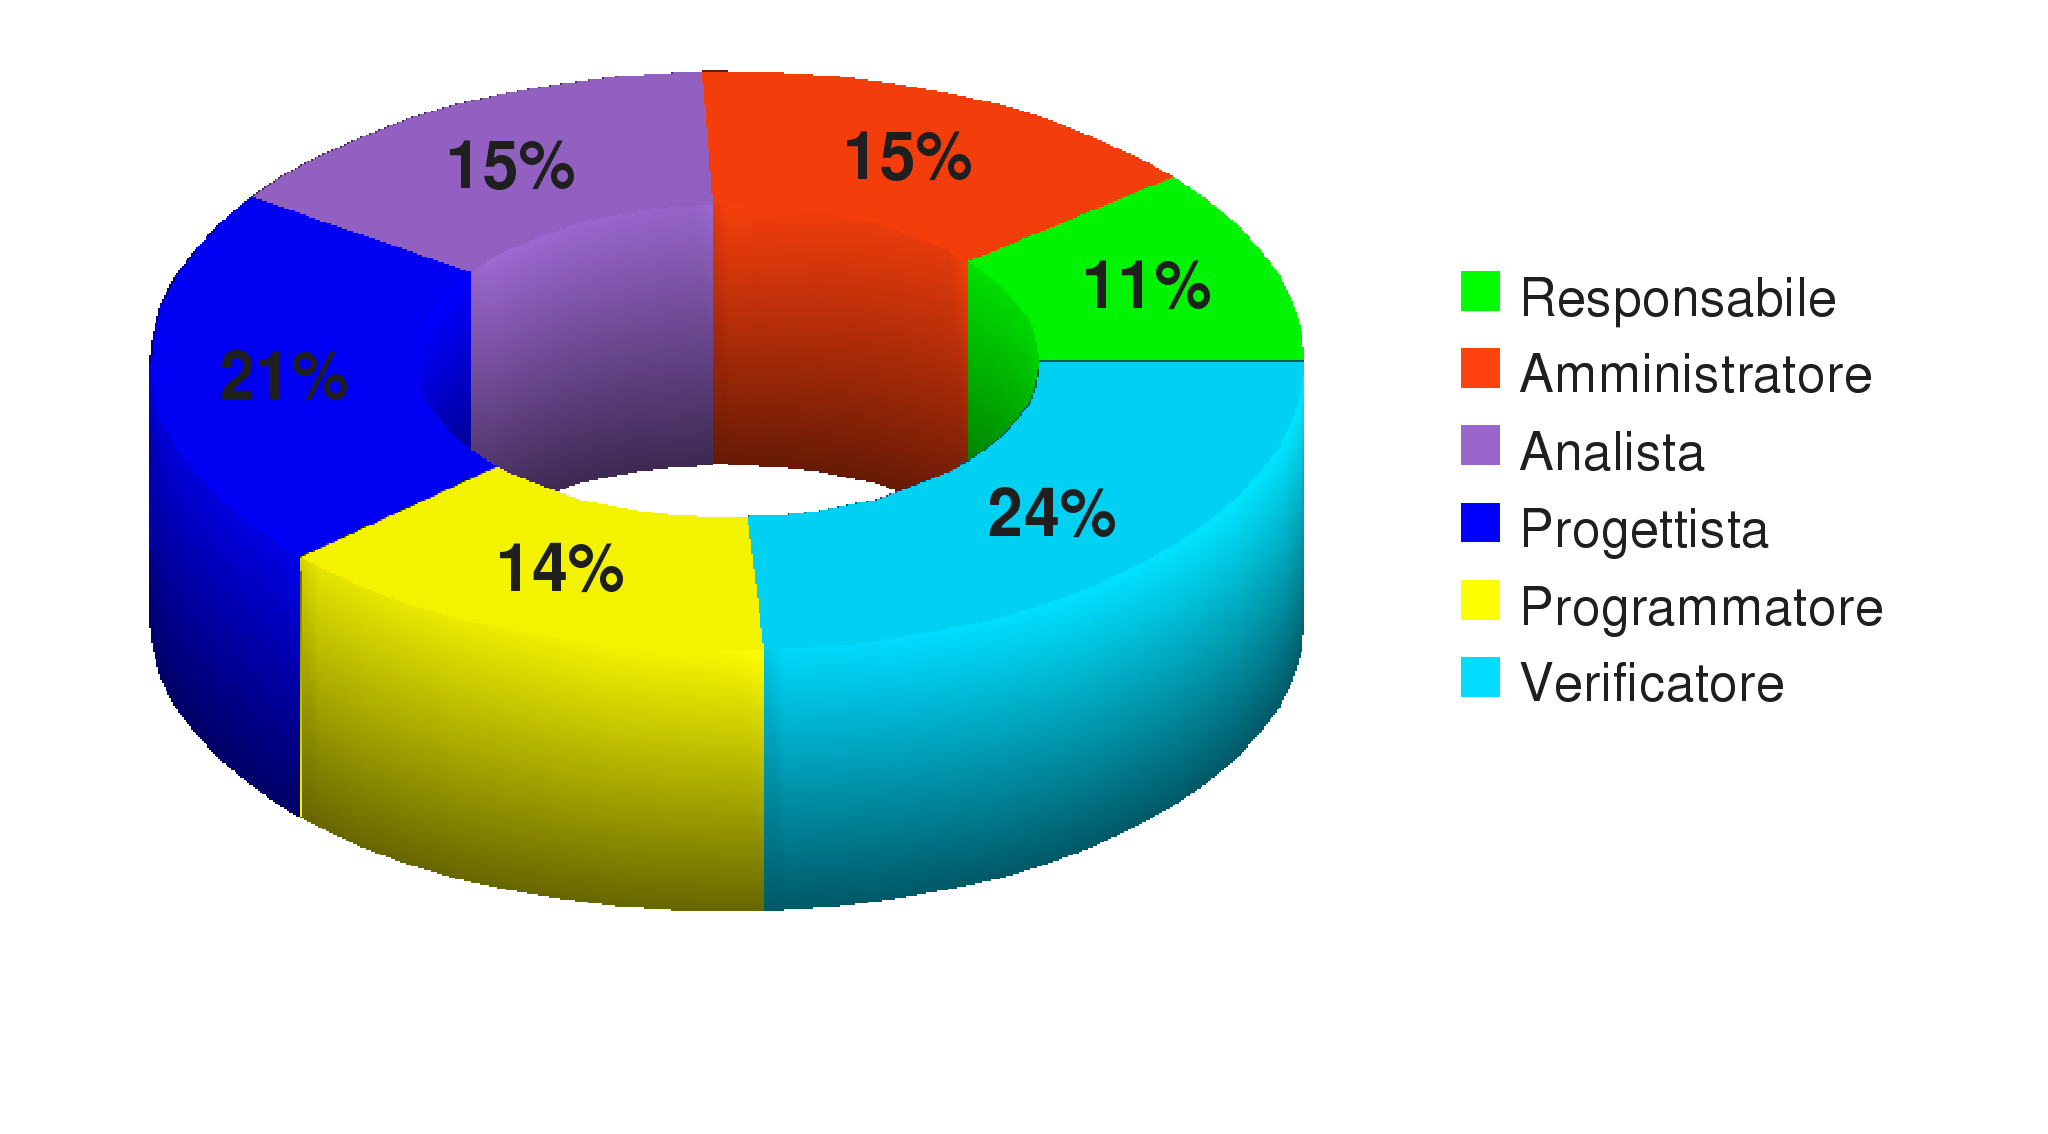
\includegraphics[width=300pt]{OreTotali}
\newpage
\begin{center}\textbf{Costo/Ruolo}
\end{center}
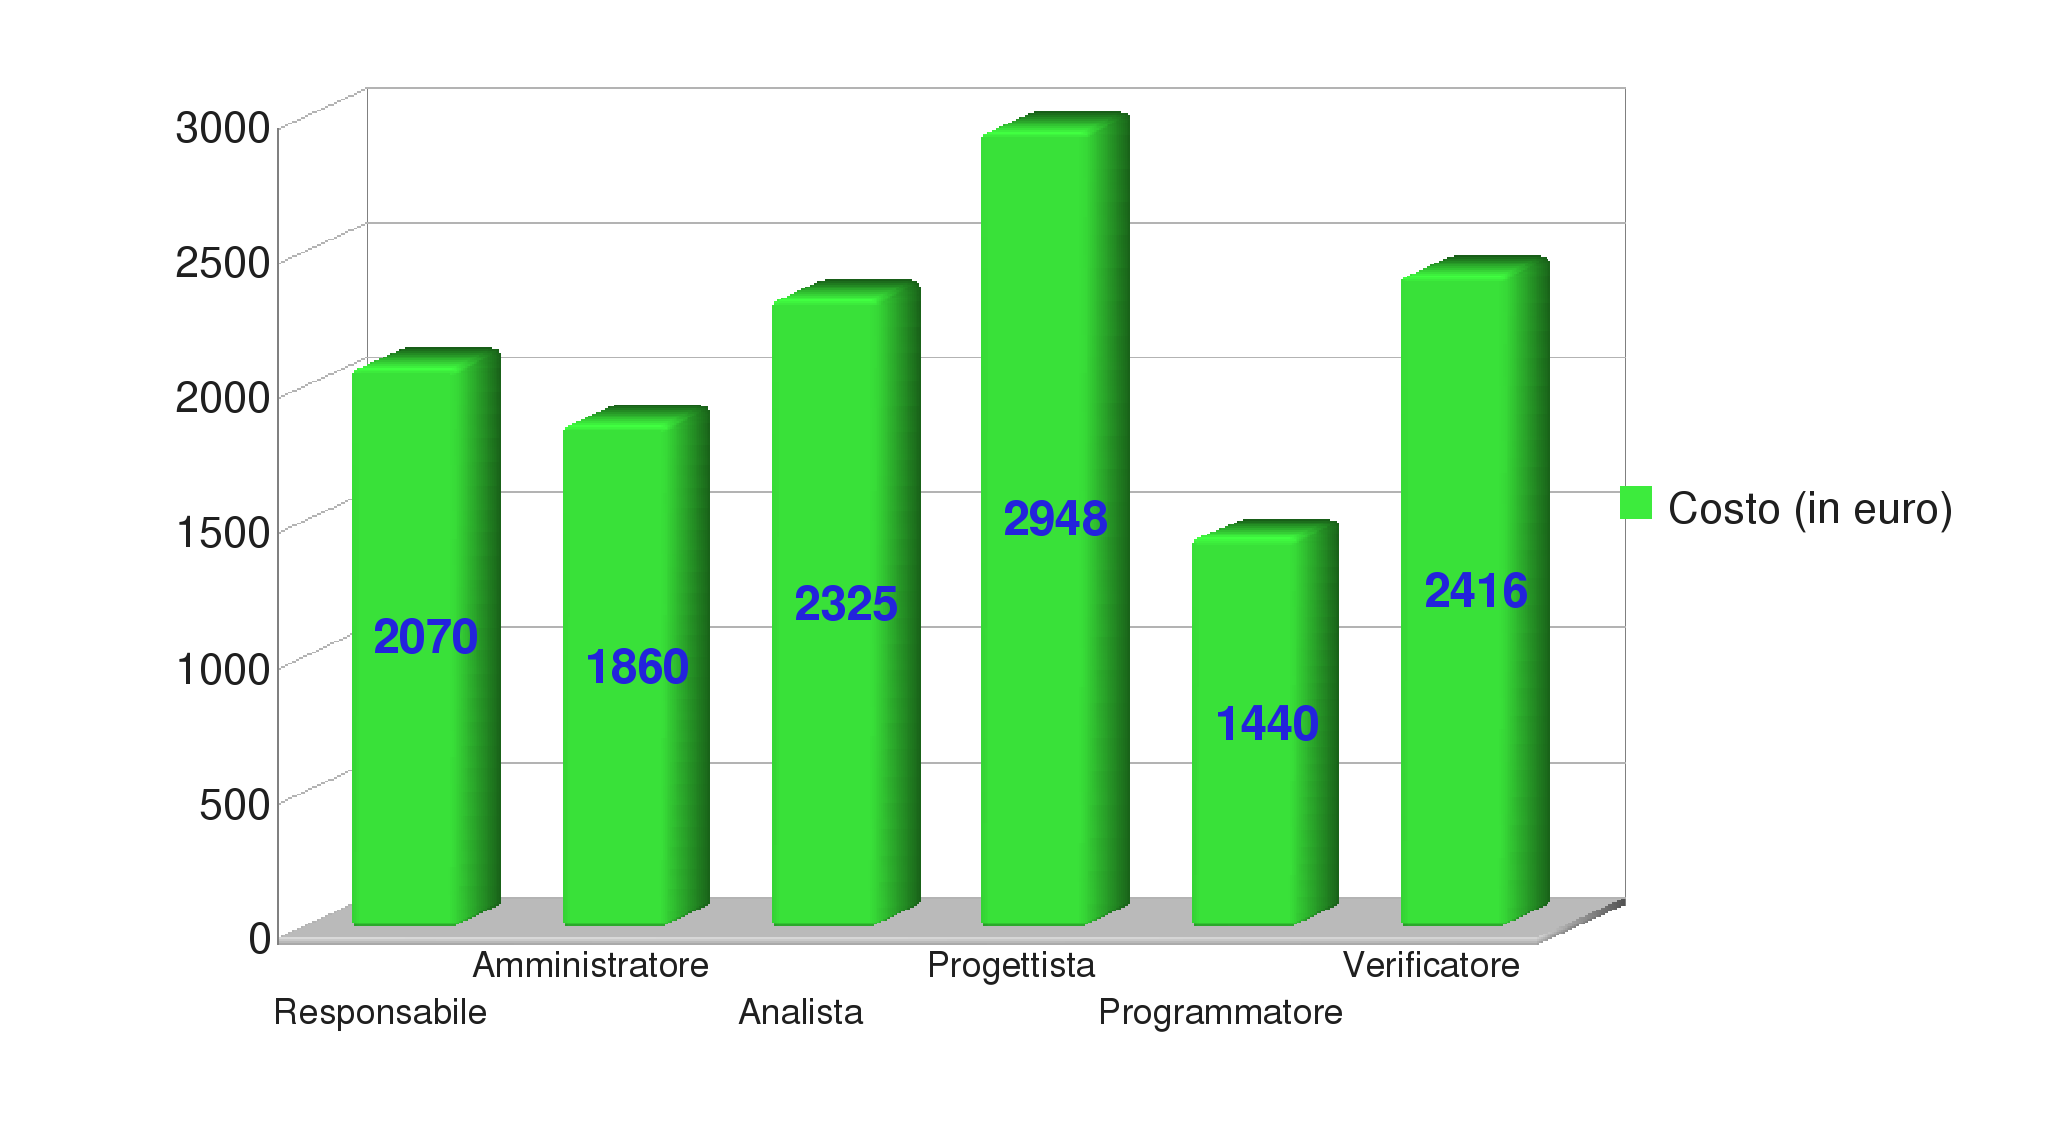
\includegraphics[width=350pt]{CostiTotali}

\subsezione{Pianificazione economico-temporale RR-RPP}
Preventivo relativo alla fase Revisione dei requisiti-Revisione del progetto preliminare.
\begin{table}[h]
	\begin{center}
		  \begin{tabular}{|c|c|c|c|}
		 \hline 
		 \textbf{Ruolo} & \textbf{Ore di lavoro} & \textbf{Costo in euro}\\
		 \hline
		Responsabile & 25 & 750 \\
		Amministratore & 40 & 800\\
		Analista & 73 & 1825\\
		Progettista & 50 & 1100\\
		Programmtore & 0 & 0 \\
		Verificatore & 35 & 560\\
        \hline
        \textbf{Totale} & \textbf{223} & \textbf{5035}\\
		\hline
		\end{tabular}
	\caption{Preventivo RR-RPP} 
	\label{tab:tabella_RR-RPP}
	\end{center}	
\end{table}


\begin{center}\textbf{Ore/Ruolo}
\end{center}
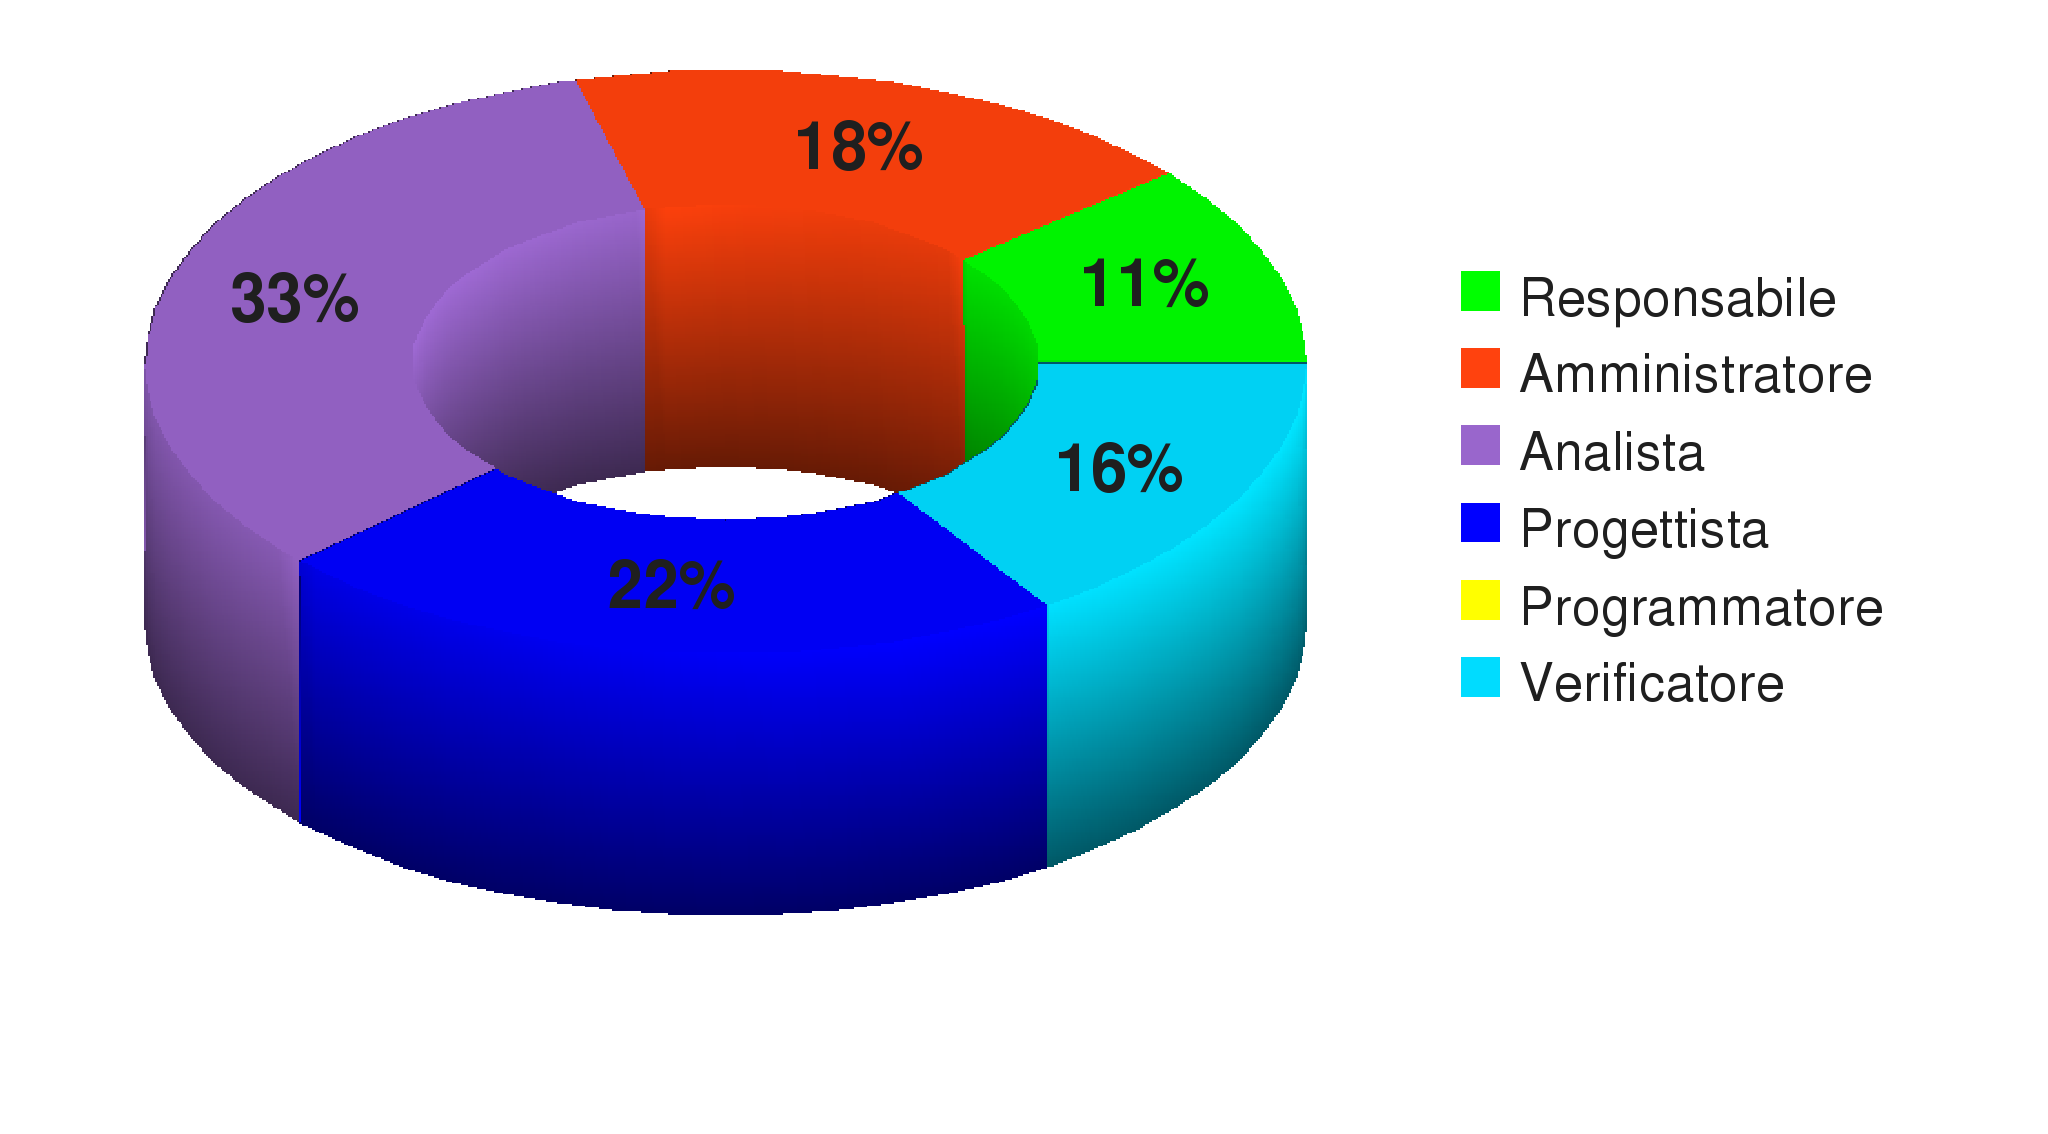
\includegraphics[width=300pt]{RR-RPP_Ore}
\newpage
\begin{center}\textbf{Costo/Ruolo}
\end{center}
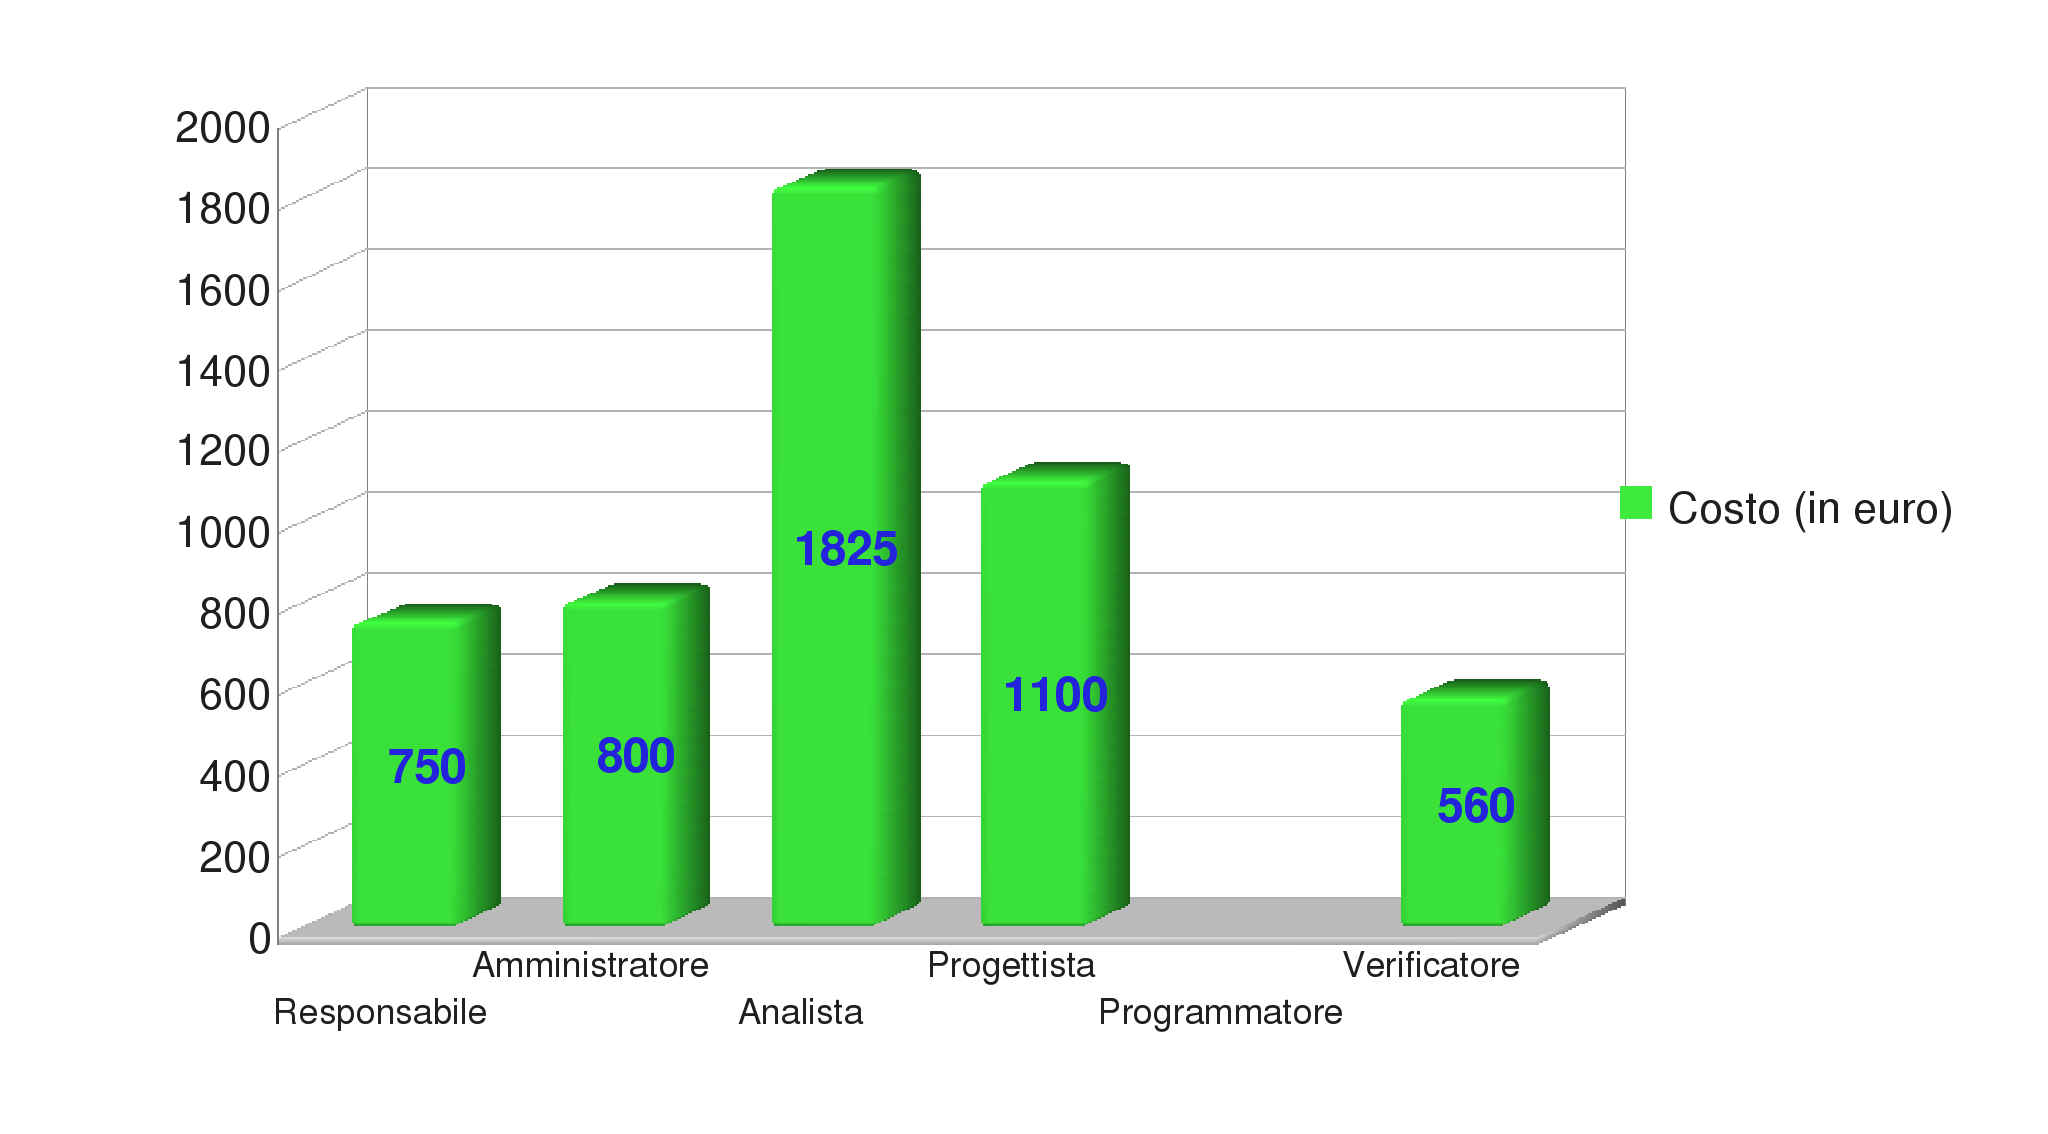
\includegraphics[width=350pt]{RR-RPP_Costi}


\subsezione{Pianificazione economico-temporale RPP-RQ}
Preventivo relativo alla fase Revisione del progetto preliminare-Revisione di qualifica.
\begin{table}[h]
	\begin{center}
		  \begin{tabular}{|c|c|c|c|}
		 \hline 
		 \textbf{Ruolo} & \textbf{Ore di lavoro} & \textbf{Costo in euro}\\
		 \hline
		Responsabile & 32 & 960 \\
		Amministratore & 35 & 700\\
		Analista & 20 & 500\\
		Progettista & 84 & 1848\\
		Programmtore & 90 & 1440 \\
		Verificatore & 101 & 1616\\
        \hline
        \textbf{Totale} & \textbf{362} & \textbf{7064}\\
		\hline
		\end{tabular}
	\caption{Preventivo RPP-RQ} 
	\label{tab:tabella_RPP-RQ}
	\end{center}	
\end{table}


\begin{center}\textbf{Ore/Ruolo}
\end{center}
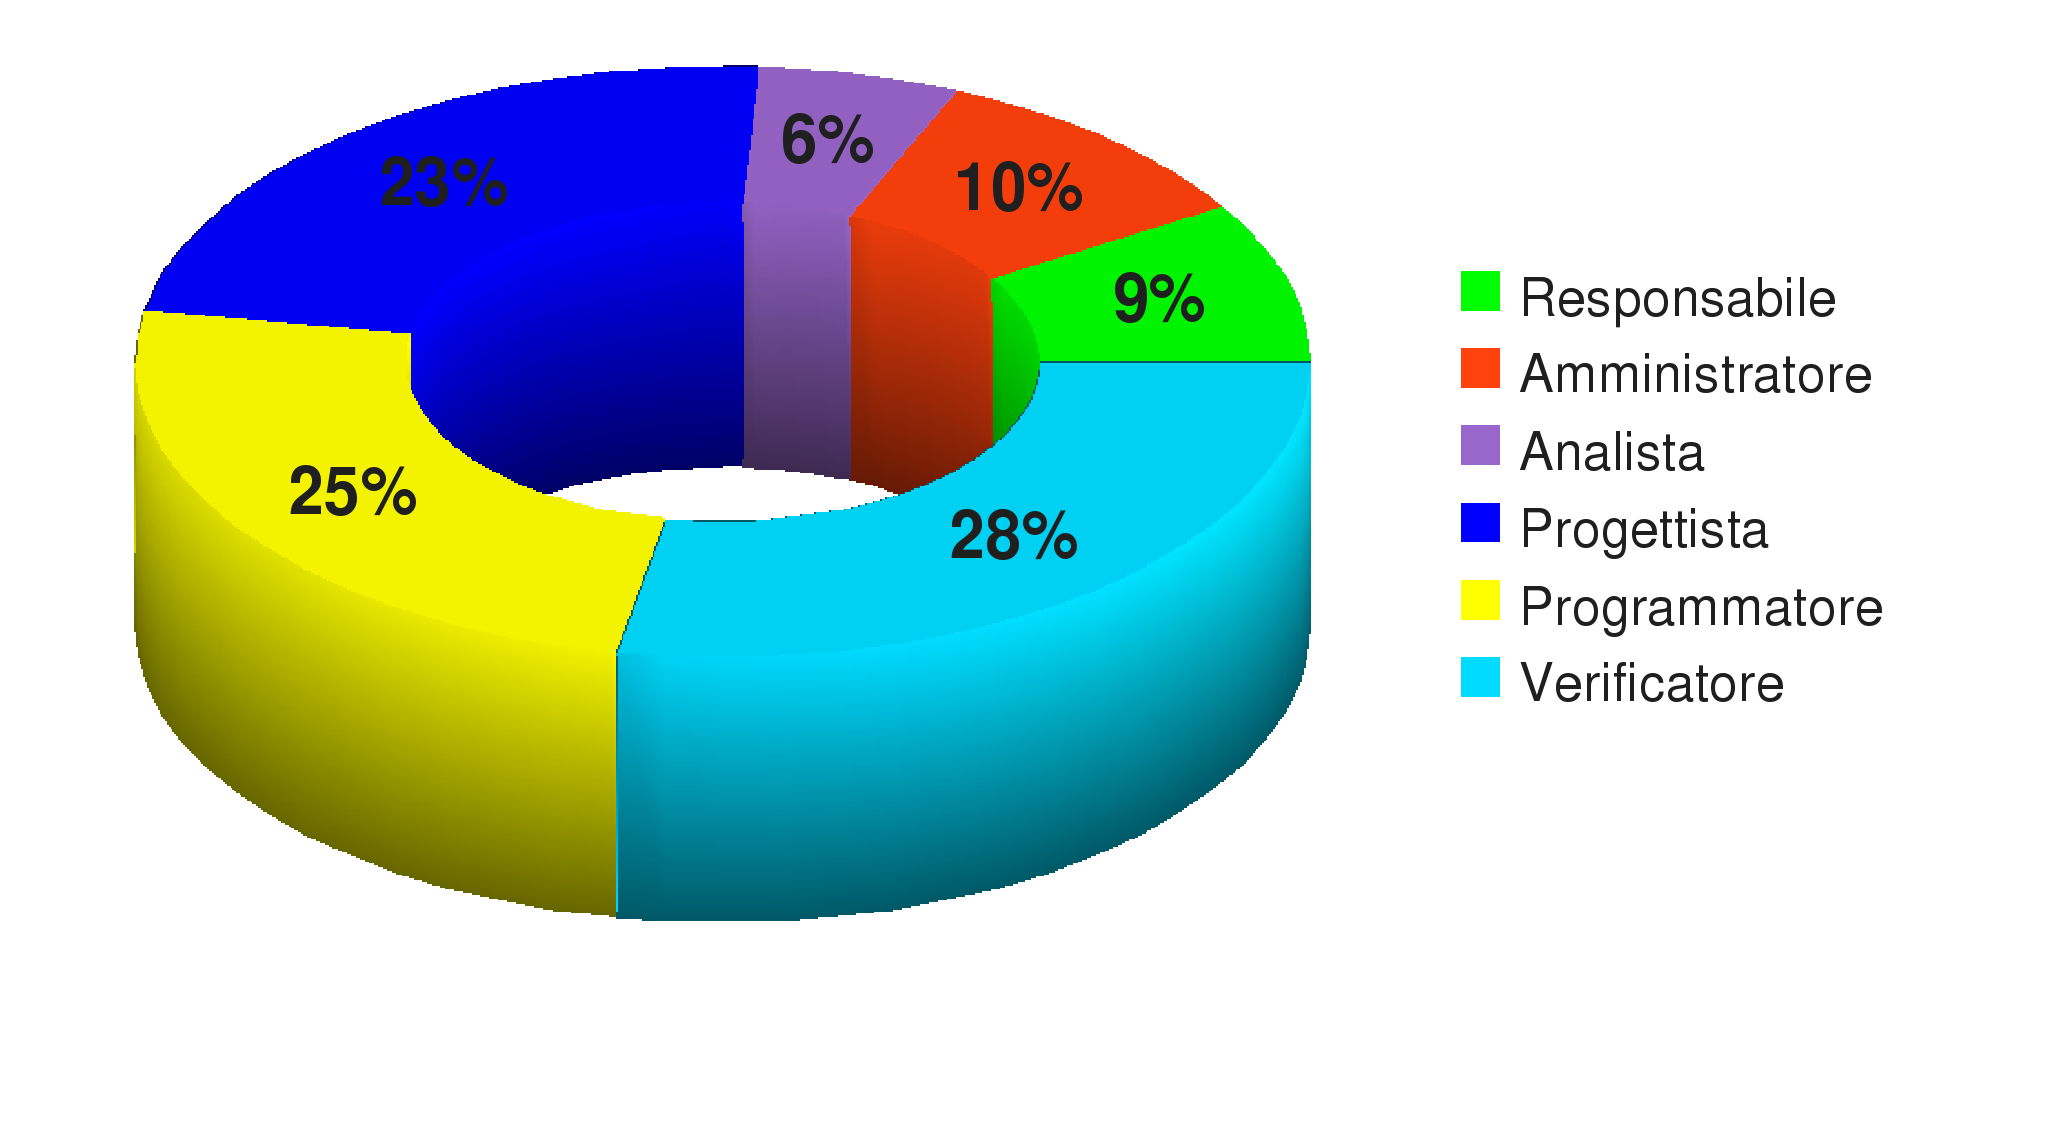
\includegraphics[width=300pt]{RPP-RQ_Ore}
\newpage
\begin{center}\textbf{Costo/Ruolo}
\end{center}
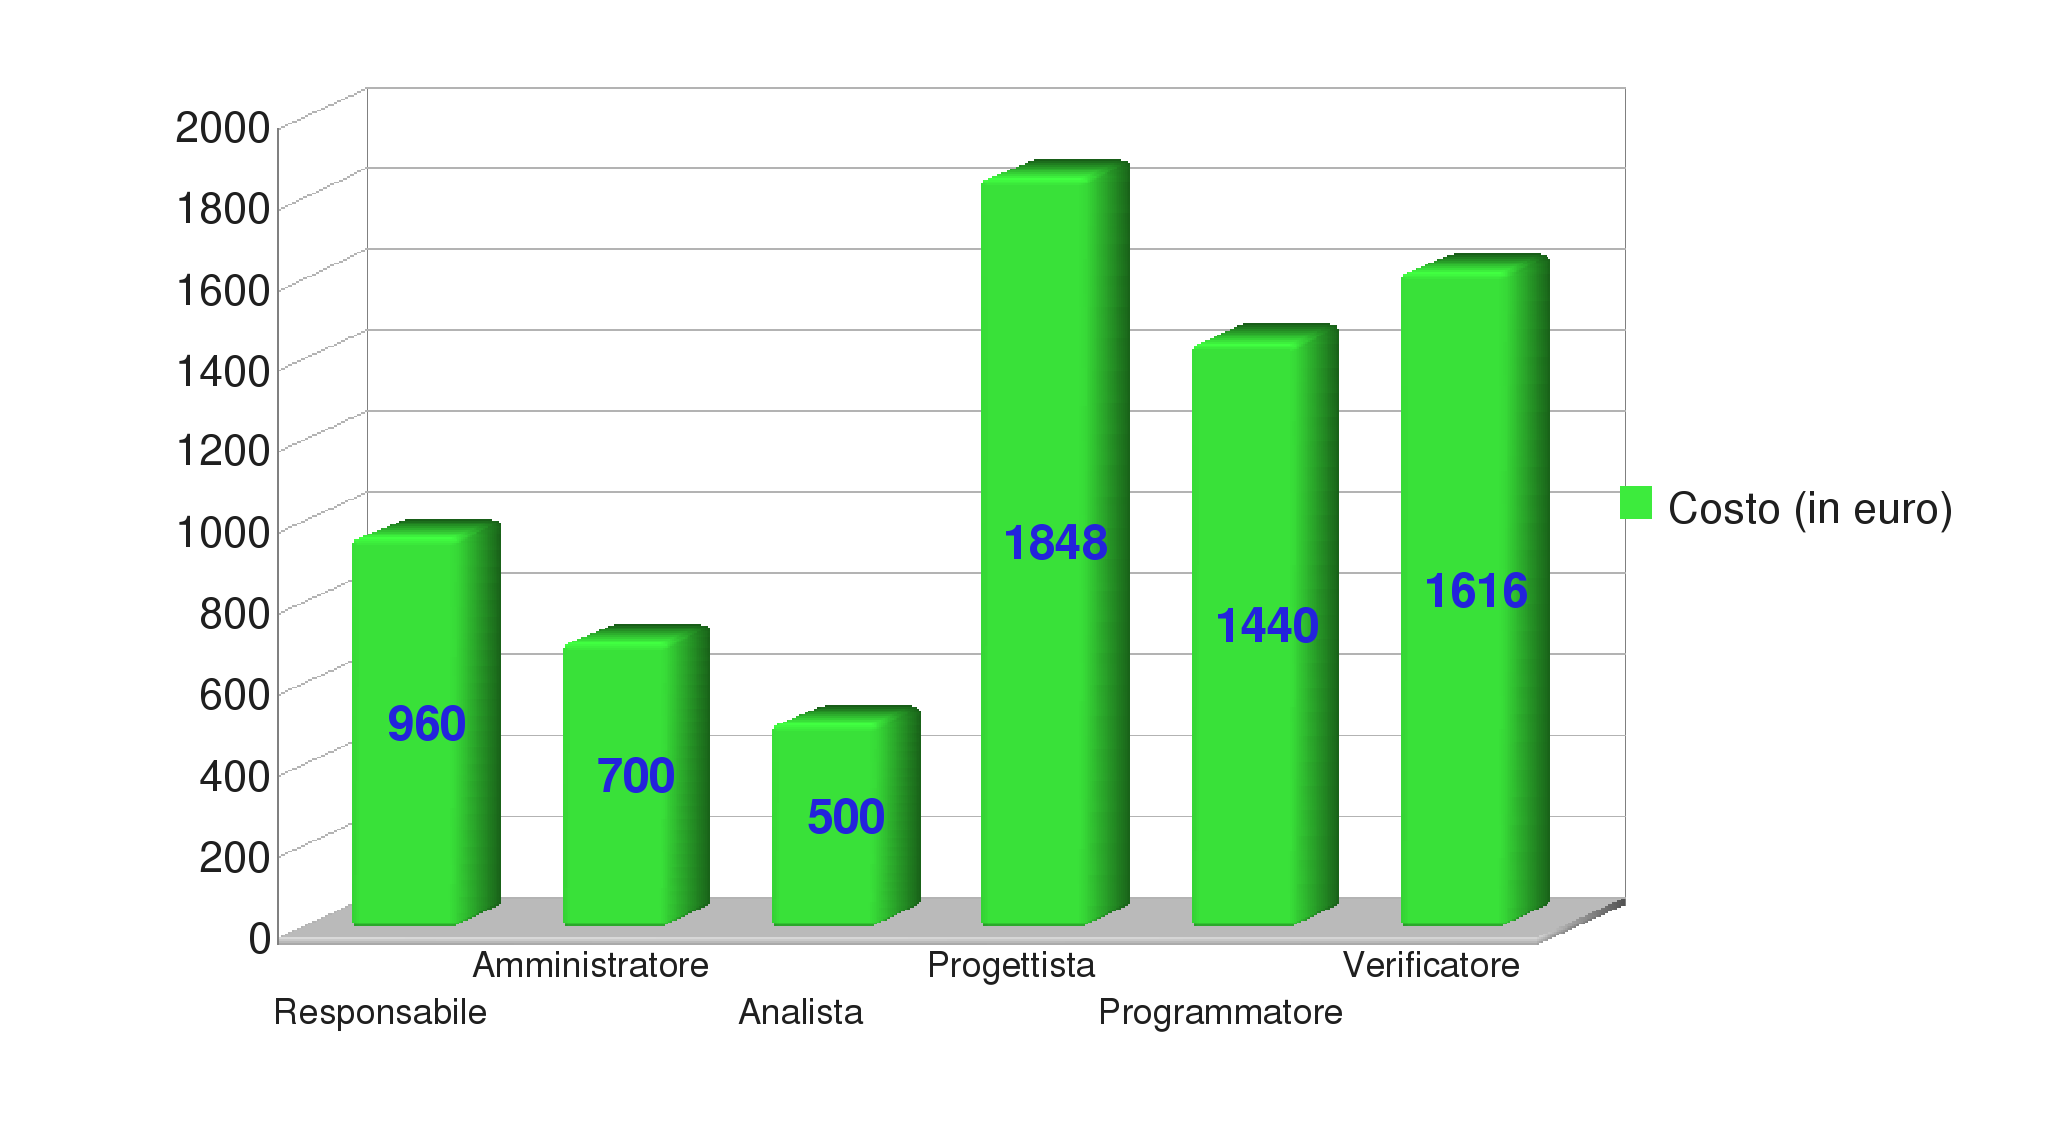
\includegraphics[width=350pt]{RPP-RQ_Costi}

\subsezione{Pianificazione economico-temporale RQ-RA}
Preventivo relativo alla fase Revisione di qualifica-Revisione di accettazione.
\begin{table}[h]
	\begin{center}
		  \begin{tabular}{|c|c|c|c|}
		 \hline 
		 \textbf{Ruolo} & \textbf{Ore di lavoro} & \textbf{Costo in euro}\\
		 \hline
		Responsabile & 12 & 360 \\
		Amministratore & 18 & 360\\
		Analista & 0 & 0\\
		Progettista & 0 & 0\\
		Programmtore & 0 & 0 \\
		Verificatore & 15 & 240\\
        \hline
        \textbf{Totale} & \textbf{45} & \textbf{960}\\
		\hline
		\end{tabular}
	\caption{Preventivo RQ-RA} 
	\label{tab:tabella_RQ-RA}
	\end{center}	
\end{table}


\begin{center}\textbf{Ore/Ruolo}
\end{center}
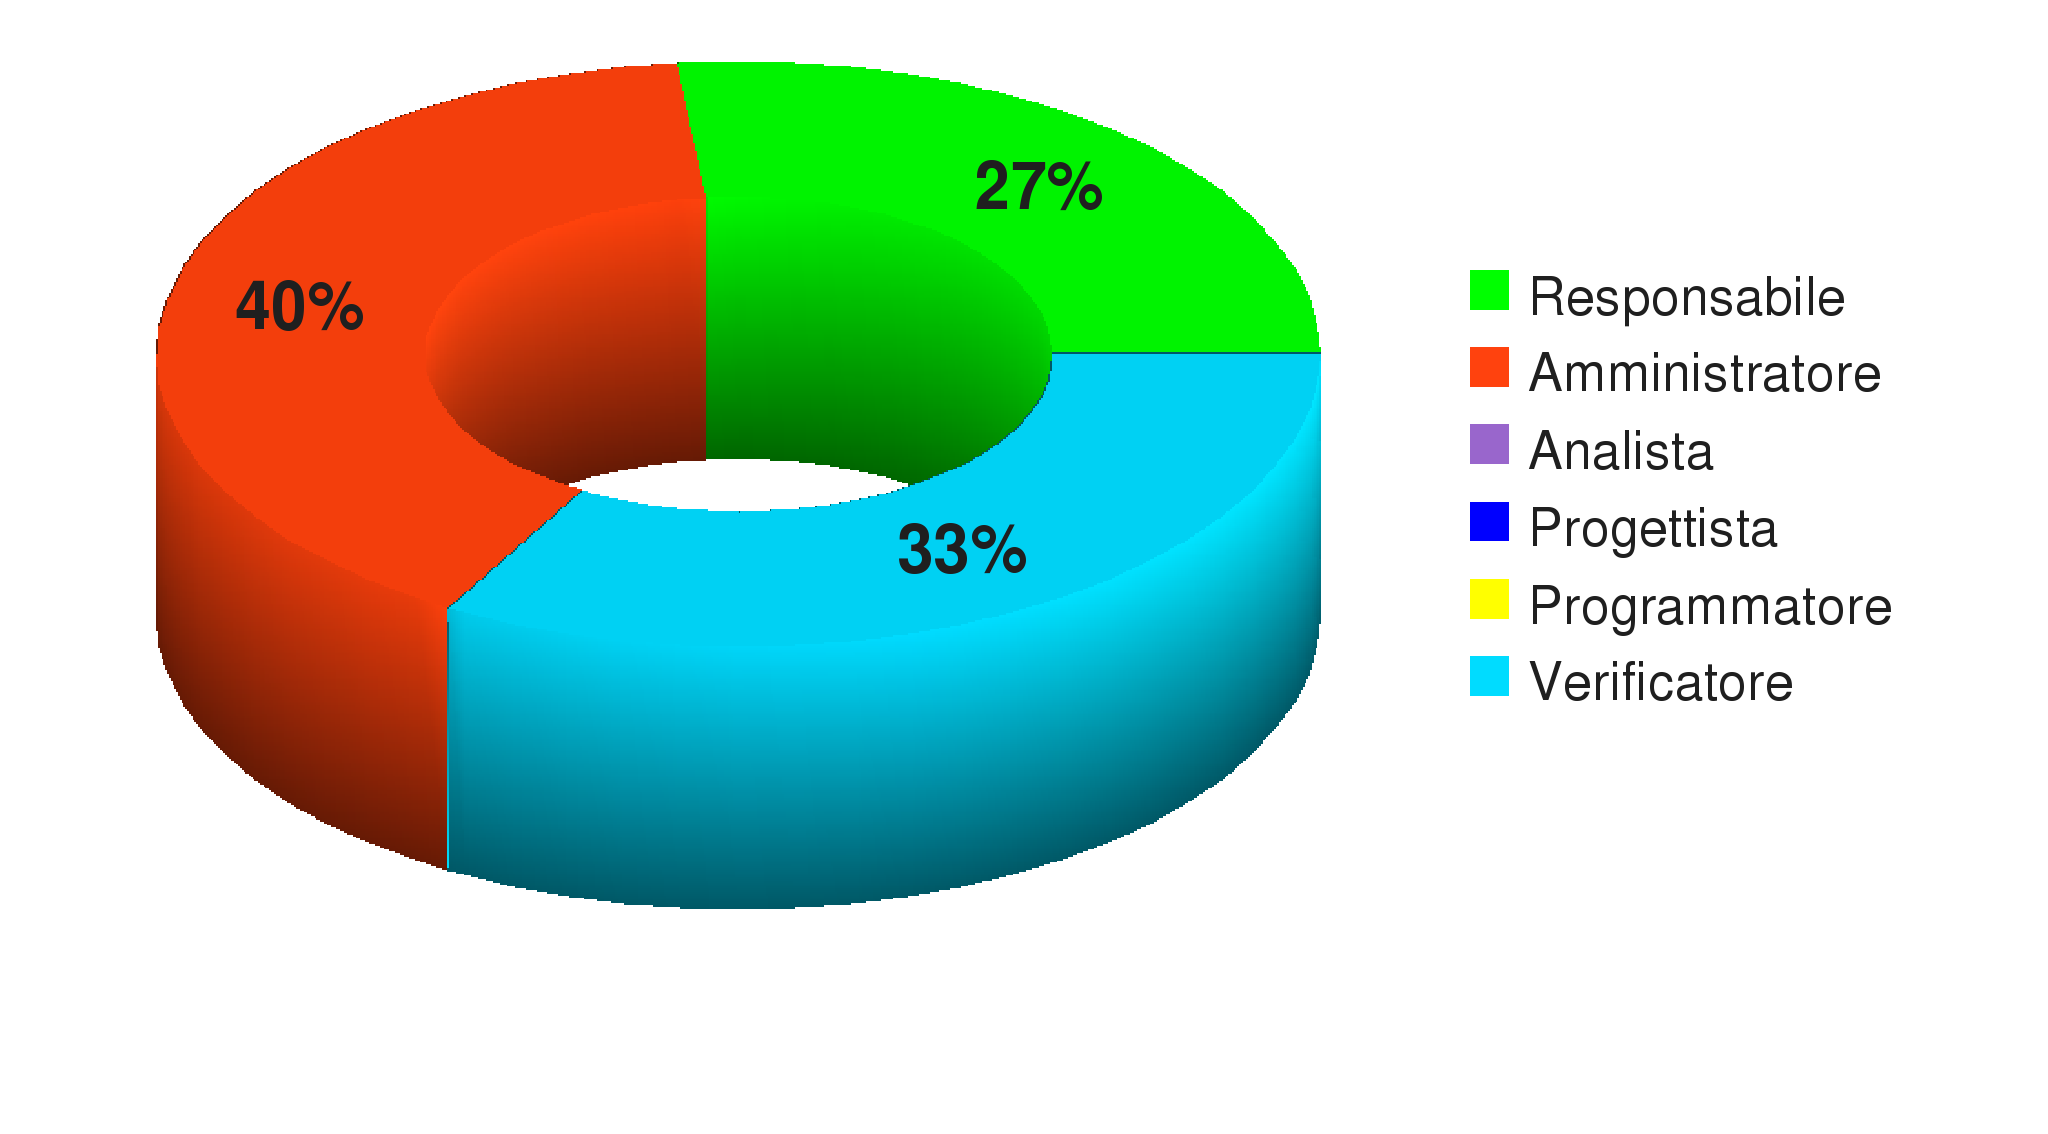
\includegraphics[width=300pt]{RQ-RA_Ore}
\newpage
\begin{center}\textbf{Costo/Ruolo}
\end{center}
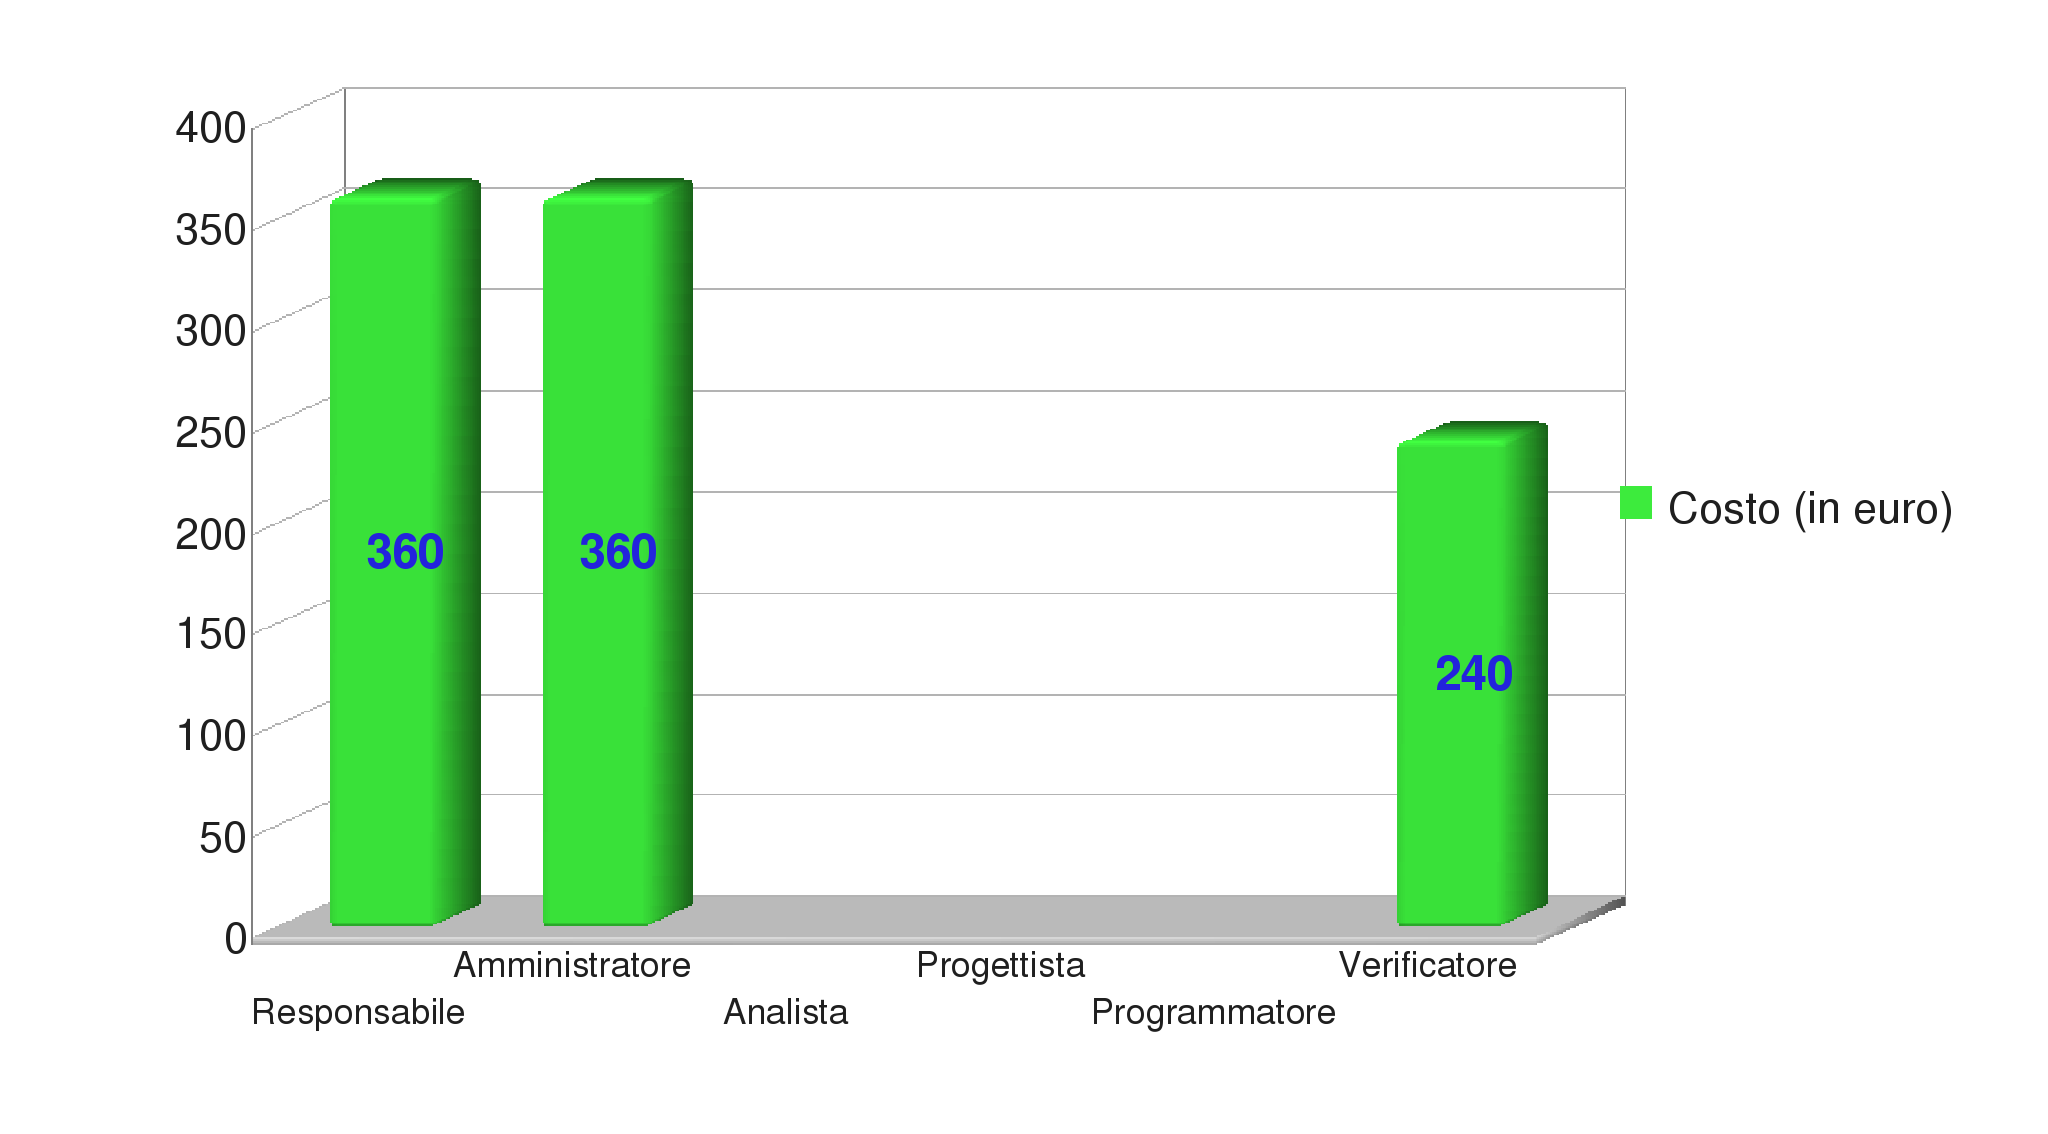
\includegraphics[width=350pt]{RQ-RA_Costi}

\subsezione{Distribuzione dei ruoli}
La distribuzione dei ruoli all'interno dell'azienda e' stata fatta in modo da dare a tutti i membri di Webshape la possibilita di ricoprire tutti i ruoli richiesti dal progetto, distribuendoli in modo piu equo possibile, rispettando i vincoli previsti dalle Assunzioni Iniziali. La distribuzione dei ruoli e' meglio descritta nella tabella (\ref{tab:TabellaRotazRuoli}) della pagina ~\pageref{tab:TabellaRotazRuoli} , e' anche descritto il carico di lavoro/persona in ore nella tabella (\ref{tab:TabellaPrevPersOre}) della pagina ~\pageref{tab:TabellaPrevPersOre}.

Per conoscenza del cliente, forniamo anche una stima approssimativa dell' impiego di ore rispetto ad ogni ruolo nella fase antecedente la RR. La remunerazione di tali ore non è a carico del committente, ma WebShape desidera mostrare quanto impegno sia stato investito nel progetto. La maggiorparte degli sforzi sono stati indirizzati al dotare Webshape di metodo di lavoro adatti allo svolgimento del progetto e per prendere confidenza con queste tecnologie.\\

\begin{table}[h]
	\begin{center}
		  \begin{tabular}{|c|c|c|c|}
		 \hline 
		 \textbf{Ruolo} & \textbf{Ore di lavoro} \\
		 \hline
		Responsabile & 20 \\
		Amministratore & 28 \\
		Analista & 65 \\
		Progettista & 10 \\
		Programmtore & 0 \\
		Verificatore & 12 \\
        \hline
        \textbf{Totale} & \textbf{135} \\
		\hline
		\end{tabular}
	\caption{Ore PRE-RR} 
	\label{tab:tabella_PRE_RR}
	\end{center}	
\end{table}

\newpage

\subsubsezione{Distribuzione per fase di progetto}
\begin{table}[!h]
	\begin{center}
		  \begin{tabular}
			  {|c|c|c|c|}
		 \hline
%%%%%%%%%%%%%%INTESTAZIONE COLONNE%%%%%%%%%%%%%%%%%%%%%%%%%%%%%%%%%%%%%%%%%%%%%%%%%%%%%%%%%%%%%%
			\multicolumn{4}{|c|}{ \textbf{Preventivo rotazione ruoli per fase di progetto} } \\
			\hline
			& \multicolumn{3}{|c|}{ \textbf{FASE} } \\
			\hline
			& \textbf{RR-RPP} & \textbf{RPP-RQ} & \textbf{RQ-RA} \\
			\hline
%%%%%%%%%%%%%%FINE INTESTAZIONE COLONNE%%%%%%%%%%%%%%%%%%%%%%%%%%%%%%%%%%%%%%%%%%%%%%%%%%%%%%%%%%%%%%
								     %  RR -RPP % RPP-RPD  %  RPD-RQ  % RQ-RA % 
			Bizzotto Piero & Resp.-Amm.-Progett.  & Analis.-Program.-Verif.   & -   \\
			\hline
			Carollo Mirko & Resp.-Amm.-Progett.  & Analis.-Program.-Verif.   \\
			\hline
			Cunico Marco & Analis.  & Resp.-Amm.-Progett.-Program.  & Verif.-Amm.   \\
			\hline
			Dal Bosco Davide & Analis.  & Resp.-Amm.-Progett.-Program.-Verif.  & -   \\
			\hline
			Dissegna Stefano & Analis.  & Resp.-Amm.-Progett.-Program.  & Verif.-Amm.   \\
			\hline
			Geremia Mirco & Resp.-Amm.-Analis.-Verif.  & Progett.-Program.  & Resp.   \\
			\hline

%%%%%%%%%%% FINE PARTE DA MODIFICARE %%%%%%%%%%%%%%%%%%%%%%%%%%%%%%%%%%%%%%%%%%%%%%%%%%%%%%%%%%%
		\end{tabular}
	\caption{Preventivo rotazione ruoli per fase di progetto} %INSERIRE DIDASCALIA - SE NECESSARIA - 
	\label{tab:TabellaRotazRuoli}
	\end{center}	
\end{table}

\subsubsezione{Distribuzione dei carichi di lavoro}
In questa sezione e' presente l'intera distribuzione del carico di lavoro per membro del gruppo.\\

\begin{table}[!h]
	\begin{center}
		  \begin{tabular}
			  {|c|c|c|c|c|c|c|}
		 \hline
%%%%%%%%%%%%%%INTESTAZIONE COLONNE%%%%%%%%%%%%%%%%%%%%%%%%%%%%%%%%%%%%%%%%%%%%%%%%%%%%%%%%%%%%%%
%			\multicolumn{3}{|c|}{ \multirow{2}{*}{ FASE RR - RPP } } \\
			\multicolumn{7}{|c|}{ \textbf{Preventivo carico persona ore} } \\
			\hline
			& \multicolumn{6}{|c|}{ \textbf{RUOLO} } \\
			\hline
			& \textbf{Resp.} & \textbf{Amm.} & \textbf{Analis.} & \textbf{Progett.} & \textbf{Program.} & \textbf{Verif.} \\
			\hline
%%%%%%%%%%%%%%FINE INTESTAZIONE COLONNE%%%%%%%%%%%%%%%%%%%%%%%%%%%%%%%%%%%%%%%%%%%%%%%%%%%%%%%%%%%%%%
								     %  RESP    % AMMIN  %  ANALISTA  %  PROGET. %  PROGRAM %    VERIF.   %
			Bizzotto Piero &  11   &  15 &  10   &   25  &  11   &  33   \\ % R4
			\hline
			Carollo Mirko &  12   &  15  &  10  &  25   &  9   &  34   \\ % R5
			\hline
			Cunico Marco    &  11   &  20  &  23   &  24   &  20   &  7   \\ % R2
			\hline
			Dal Bosco Davide        &  10   &  15   &  10   &  21   &   15  &  34  \\ % R1
			\hline
			Dissegna Stefano        &  11  &  18   & 22  &  26   &  20  &  8  \\ % R6
			\hline
			Geremia Mirco   &   14  &  10   &  18   &  13  &  15   &  35   \\ % R7
			\hline		
%%%%%%%%%%% FINE PARTE DA MODIFICARE %%%%%%%%%%%%%%%%%%%%%%%%%%%%%%%%%%%%%%%%%%%%%%%%%%%%%%%%%%%
		\end{tabular}
	\caption{Preventivo carico persona in ore} %INSERIRE DIDASCALIA - SE NECESSARIA - 
	\label{tab:TabellaPrevPersOre}
	\end{center}	
\end{table}

\sezione{Gestione del Piano di Progetto}
\subsezione{Obiettivi}
L'obiettivo del documento denominato "Piano di Progetto" \`e di distribuire le risorse durante l'arco temporale 
contenente lo sviluppo del capitolato d'appalto. Questa distribuzione ovviamente deve rispettare i vincoli presentati 
nella sezione "Assunzioni Iniziali".

\sezione{Analisi e Gestione dei Rischi}
In questa sezione saranno presi in considerazione i possibili problemi che potrebbero sorgere durante la realizzazione del progetto, sia dal punto di vista della pianificazione delle fasi di lavoro, che da eventuali rischi relativi alla tecnologia usata.\\
I punti di rischio da noi identificati e valutati sono i seguenti:
\begin{itemize}
\item \textbf{Rischi inerenti al modello di ciclo di vita evolutivo}\\
\`e molto importante effettuare una corretta scelta delle attivit\`a, da coordinare durante le varie fasi di lavoro.\\
\item \textbf{Pianificazione e distribuzione dei ruoli}\\ 
un punto fondamentale al quale bisogna prestare molta attenzione \`e la suddivisione dei ruoli e la sua gestione. Ogni componente dovr\`a assumere tutti i ruoli durante le varie fasi di progetto. Questo pu\`o portare ad una scarsa specializzazione dei membri dell'azienda, ma \`e un vincolo didattico indispensabile.
\item \textbf{Mancanza del personale}\\
essendo l'azienda formata da sei membri, nell'eventualit\`a che un membro non possa pi\`u partecipare alle attivit\`a di progetto, c'\`e un possibile rischio che l'azienda abbia un numero insufficiente di persone per continuare il lavoro sotto le ipotesi e le stime preventivate. In questo caso, l'azienda WebShape porter\`a comunque a termine il suo lavoro.\\
\item \textbf{Compatibilit\`a e portabilit\`a del prodotto}\\
il prodotto finale, come da Requisiti, deve essere funzionante sui pi\`u moderni browser in circolazione. Questo per\`o \`e un fatto a discrezione dell'utente finale, il quale deve essere consapevole e informato che il prodotto non \`e retrocompatibile e quindi anche la portabilit\`a \`e a sua discrezione.
\item \textbf{Funzionalit\`a del prodotto}\\
essendo il prodotto finale utilizzato da un qualsiasi tipo di utente finale, \`e necessario prestare attenzione a come il prodotto si presenta, rendendo l'accessibilit\`a a tutte le sue funzioni semplice e immediata.
\end{itemize}			

da completare\\

\end{document}
